\documentclass{beamer}
\usepackage{amsfonts,amsmath,oldgerm}
\usepackage{ragged2e}

\usetheme{sintef}

\newcommand{\testcolor}[1]{\colorbox{#1}{\textcolor{#1}{test}}~\texttt{#1}}

\usefonttheme[onlymath]{serif}

\titlebackground*{assets/background}

\newcommand{\hrefcol}[2]{\textcolor{cyan}{\href{#1}{#2}}}

\title{Aula Zero - Programa da Disciplina}
\subtitle{2023.1 - SPOSOPE -  Sistemas Operacionais}
\course{Tecnologia em Análise e Desenvolvimento de Sistemas}
\author{\href{mailto:luiz.quirino@ifsp.edu.br}{Luiz \textbf{Quirino}}}
\IDnumber{luiz.quirino@ifsp.edu.br}



\begin{document}
\maketitle

%\begin{frame}
%
%      Este material é produzido utilizando \LaTeX\, baseado na SINTEF Presentation, disponibilizado sob licenciamento \hrefcol{https://creativecommons.org/licenses/by-nc/4.0/legalcode}{Creative Commons CC BY 4.0}
%
%\vspace{\baselineskip}

%In the following you find a brief introduction on how to use \LaTeX\ and the beamer package to prepare slides, based on the one written by \hrefcol{mailto:federico.zenith@sintef.no}{Federico Zenith} for \hrefcol{https://www.overleaf.com/latex/templates/sintef-presentation/jhbhdffczpnx}{SINTEF Presentation}

% This template is released under \hrefcol{https://creativecommons.org/licenses/by-nc/4.0/legalcode}{Creative Commons CC BY 4.0} license
%\end{frame}
\footlinecolor{sintefdarkgreen}
\section{Apresentação docente}

\begin{frame}{Sobre o docente:}
Formação:
\begin{itemize}
\item Pós-graduação em Gestão de Riscos e CiberSegurança - Faculdade Focus
\item Sistemas de Informação - UFMS
\item Gestão de Tecnologia da Informação - Unicesumar
\item Técnico em Informática - Centro Paula Souza
\end{itemize}
Áreas de Interesse:
\begin{itemize}
\item Gestão de Tecnologia da Informação
\item Governança de Tecnologia da Informação
\item Gestão de Riscos e CiberSegurança
\item Desenvolvimento de software
\end{itemize}
\end{frame}

\section{Apresentação da disciplina}

\begin{frame}{Ementa}\justifying
      A disciplina aborda o conjunto de programas usados para gerenciar recursos de computadores, fornecendo uma interface com o usuário. 
      São trabalhos os fundamentos, instalação e configuração de sistemas operacionais e aplicativos modernos, gestão de armazenamento, 
      usuários e processos de software, proporcionando ao estudante, habilidade para selecionar
      e instalar sistemas operacionais e programas de computador adequados as necessidades 
      de usuários e empresas, e instalar seu próprio computador de desenvolvimento.
\end{frame}

\begin{frame}{Objetivo da disciplina}\justifying
      Identificar os fundamentos de sistemas operacionais modernos e a sua importância para sistemas de informação. Conhecer os mecanismos internos a um sistema operacional. Selecionar, instalar e configurar sistemas operacionais. Comparar e aplicar diferentes soluções de sistemas operacionais.
\end{frame}

\begin{frame}{Conteúdo Programático}\justifying
      \begin{itemize}
            \item Fundamentos de Sistemas Operacionais
                  \begin{itemize}
                        \item História dos sistemas operacionais modernos 
                        \item Processos, memoria, arquivos, entrada/saída e proteção
                        \item Chamadas de sistema
                        \item Estrutura de um SO
                  \end{itemize}
            
            
      \end{itemize}
\end{frame}

\begin{frame}{Conteúdo Programático}\justifying
      \begin{itemize}
            \item Particionamento de disco e instalação de sistema operacional para Desktop em máquina virtual
            \item Processo de inicialização
            \item Operações em diretórios e arquivos, Filesystem Hierarchy Standard (FHS)
            \item Comandos para manipulação de arquivos texto
            \item Permissões e propriedades de arquivos e diretórios
            \item Programação de scripts shell, parâmetros de entrada, variáveis de ambiente
           
      \end{itemize}
\end{frame}

\begin{frame}{Conteúdo Programático}
      \begin{itemize}
          \item Agrupamento e compressão de arquivos
          \item Sistemas gerenciadores de pacotes
          \item Gerenciamento de entrada e de saída
          \item Gerenciamento de pacotes, aplicativos externos à distribuição
          
      \end{itemize}
  \end{frame}

  \begin{frame}{Conteúdo Programático}
      \begin{itemize}
         
          \item Gerenciamento de processos
              \begin{itemize}
                  \item Escalonamento de processos
                  \item Interrupções de hardware
                  \item Ciclo de vida de processos
                  \item Comunicação interprocessos
              \end{itemize}
          
      \end{itemize}
  \end{frame}
  
  \begin{frame}{Conteúdo Programático}
      \begin{itemize}
          
          \item Gerenciamento de memória
              \begin{itemize}
                  \item Memória virtual
                  \item Semáforos
                  \item Concorrência
                  \item Threads
              \end{itemize}
          
      \end{itemize}
  \end{frame}

  \begin{frame}{Conteúdo Programático}
      \begin{itemize}
         
          \item Introdução e prevenção de deadlocks
          \item Gerenciando usuários, grupos e permissões
          \item Comandos para analisar partições e sistema de arquivos
          \item Comandos para analisar o desempenho
      \end{itemize}
  \end{frame}

\begin{frame}{Bibliografia básica}\justifying
      \begin{itemize}
            \item \textbf{DEITEL, Harvey M.; DEITEL, Paul J.; CHOFFNES, David R.\textcolor{sintefdarkgreen}{ Sistemas operacionais. 3. ed.}} São Paulo: Pearson Education, 2005. ISBN 9788576050117. Disponível em: https://ifsp.bv3.digitalpages.com.br/users/publications/9788576050117. Acesso em: 14 jun. 2019.

            \item \textbf{OLIVEIRA, Rômulo Silva de; CARISSIMI, Alexandre da Silva; TOSCANI, Simão Sirineo.\textcolor{sintefdarkgreen}{ Sistemas operacionais. 1. ed.}} Porto Alegre: Bookman, 2010. ISBN 9788577805211.
        
            \item \textbf{TANENBAUM, Andrew S.; BOS, Herbert.\textcolor{sintefdarkgreen}{ Sistemas operacionais modernos. 4. ed.}} São Paulo: Pearson Education do Brasil, 2016. ISBN 9788543005676. Disponível em: https://ifsp.bv3.digitalpages.com.br/users/publications/9788543005676. Acesso em: 14 jun. 2019.
        
      \end{itemize}
\end{frame}
      

\begin{frame}{Bibliografia complementar}
      \begin{itemize}
            \item \textbf{ENGLANDER, Irv.} A arquitetura de hardware computacional, software de sistema e comunicação em rede: uma abordagem da tecnologia da informação. 4. ed. Rio de Janeiro: LTC, 2011. ISBN 9788521617917.

            \item \textbf{FLYNN, Ida; MCHOES, Ann McIver.} Introdução aos sistemas operacionais. 1. ed. São Paulo: Cengage Learning, 2002. ISBN 9788522102740.
        
            \item \textbf{MACHADO, Francis Berenger; MAIA, Luiz Paulo.} Arquitetura de sistemas operacionais. 5. ed. Rio de Janeiro: LTC, 2013. ISBN 9788521622104.
        
            \item \textbf{SILBERSCHATZ, Abraham; GALVIN, Peter Baer; GAGNE, Greg.} Sistemas operacionais com java. 8. ed. Rio de Janeiro: Elsevier, 2016. ISBN 9788535283676.
        
            \item \textbf{TANENBAUM, Andrew S.; WOODHULL, Albert S.} Sistemas operacionais: projeto e implementação. 3. ed. Porto Alegre: Bookman, 2008. ISBN 9788577800571.
      \end{itemize}
\end{frame}



\section{Planejamento}


\begin{frame}[fragile]{Planejamento de aulas}
      \begin{columns}
            \begin{column}{0.5\textwidth}
                  \textbf{Definições da disciplina:}
                  \begin{itemize}
                        \item Total de aulas: 95 
                        \item Aulas semanais: 5 (19 semanas)
                        \item Total de horas: 71,25
                        \item Atividades práticas
                        \item Atividades teoricas (discussões e questionários)
                        \item Provas teóricas
      
                  \end{itemize}


            \end{column}
            \begin{column}{0.5\textwidth}
                  \textbf{Turma: 324025}
                  \begin{itemize}
                        \item Quartas-feiras: 18:50 - 22:50
                        \item Período: 02/08 - 29/11 → IFA)
                        \item Feriados: 15/11
                        \item Eventos: 20/09
                  \end{itemize}
                  
            \end{column}
      \end{columns}
\end{frame}



%\section{Moodle}

%\begin{frame}[fragile]{Auto Inscrição Moodle}
%
%      \textbf{Autoinscrição → \textcolor{sintefred}{Chave: IFSP@2023.2}}
%
%      \begin{figure}[H]
%            \centerline{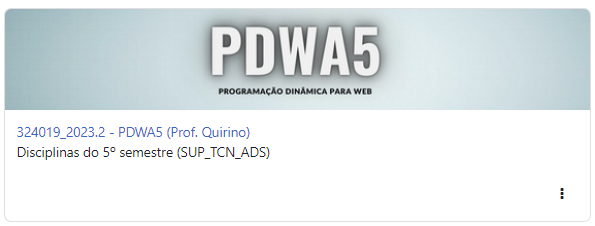
\includegraphics[width=1\textwidth]{assets/aula-tads-pdwa5/moodle_quinta.png}}
%            
%        \end{figure}
%        
%\end{frame}


\section{Avaliações}

\begin{frame}[fragile]\justifying
\frametitle{Sistema de avaliação}
\begin{itemize}
            
            \item Como seremos avaliados:
            \begin{itemize}
                  \item Duas provas teóricas atendendo a 65\% da nota;
                  \item Atividades avaliativas diversas, contando como 35\% da nota;
            \end{itemize}
            \item Em caso de não obtenção dos critérios mínimos para aprovação, aplicação de IFA por meio de prova teórica, escrita, presencial;
\end{itemize}


\end{frame}


\begin{frame}[fragile]\justifying
      \frametitle{Sistema de avaliação}
      \begin{itemize}
            \item Média prova \[ MP = ( P1 + P2 ) * 0,65 \]
            \item Média atividade \[ MA = \left ( \frac{A_1 + A_2 + ... + A_n}n \right ) * 0,35 \]
            \item Média Final - MF \[MF = MP + MA\]
      \end{itemize}
      
      \end{frame}
      \footlinecolor{}

\begin{frame}[fragile]\justifying
      \frametitle{Critérios de avaliação}
      Respeitando ao disposto no PPC vigente do curso, no item \textbf{\textit{8. AVALIAÇÃO DA APRENDIZAGEM. }}
      \newline
      \newline
      \textit{Os critérios de aprovação nos componentes curriculares, envolvendo simultaneamente frequência e avaliação, para os cursos da Educação Superior de 
      regime semestral, são a obtenção, no componente curricular, de nota semestral igual ou superior a 6,0 (seis) e frequência mínima de 75\% (setenta e cinco por cento) das
      aulas e demais atividades. }
\end{frame}

\begin{frame}[fragile]\justifying
      \frametitle{Critérios de avaliação}
      \textit{Fica sujeito ao Instrumento Final de Avaliação (IFA), o estudante que obtenha, no componente curricular, nota semestral igual ou superior a
      4,0 (quatro) e inferior a 6,0 (seis) e frequência mínima de 75\% (setenta e cinco por cento) das aulas e demais atividades. O estudante que realizar o Instrumento Final de
      Avaliação, para ser aprovado, deverá obter a nota mínima igual a 6,0 (seis). A nota final considerada, para registros escolares, será a maior entre a nota semestral e a nota do
      Instrumento Final de Avaliação (IFA). 
      \newline
      \newline
      É importante ressaltar que os critérios de avaliação na Educação Superior primam pela autonomia intelectual.}
\end{frame}

\section{Conduta ética}
\begin{frame}
\frametitle{Termos de Conduta}
      \begin{itemize}
            \item Trabalhos e provas devem ser feitas INDIVIDUALMENTE;
            \item Cada estudante tem responsabilidade sobre cópias de suas implementações e provas, mesmo que parciais;
            \item Não faça implementeções em grupo e não compartilhe programas ou trechos de programas;
            \item Você pode consultar seus colegas para esclarecer dúvidas e discutir idéias sobre implementações, mas NÃO copie programas!
            \item Implementações e provas consideradas plagiadas terão nota ZERO;
            \item O estudante que se envolver em DOIS CASOS DE PLÁGIO estará automaticamente REPROVADO na disciplina.
      \end{itemize}
\end{frame}

\section{Informações sobre os slides}

\footlinecolor{sintefyellow}
\begin{frame}[fragile]{Dicas sobre os slides}
      
      \begin{itemize}
            \item Slides com rodapé em vermelho foram adicionados após a aula dada;
            \item Slides com rodapé em amarelo foram atualizados  após a aula dada.
      \end{itemize}
\end{frame}

\footlinecolor{sintefred}
\begin{frame}[fragile]{Imagem do dia}

        \begin{figure}[H]
            \centerline{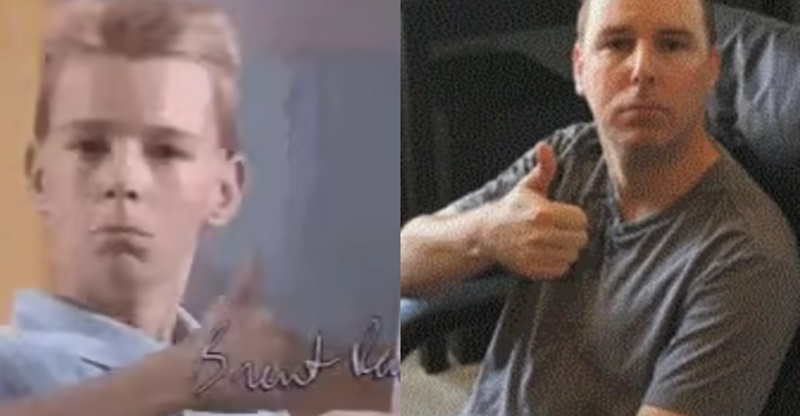
\includegraphics[width=0.8\textwidth]{assets/imagem-do-dia/brent_rambo.jpg}}
            
        \end{figure}
\end{frame}


\footlinecolor{}

\backmatter
\end{document}
